\documentclass[
	english,
        solution=true
	]{tudaexercise}

\usepackage[main=english, ngerman]{babel}
\usepackage[babel]{csquotes}

\usepackage{amstext}
\usepackage{amsmath}
\usepackage{amssymb}
\usepackage{graphicx}
\usepackage{setspace}
\usepackage{multicol}
\usepackage{mathtools}
\usepackage{dsfont}
\usepackage{units}
\usepackage{subfigure}
\usepackage{color}
\usepackage{booktabs}
\usepackage{fancyref}
\usepackage{listings}
\usepackage{mathrsfs}
\usepackage{physics}
\usepackage{gauss}
\usepackage{bm}
\usepackage{multirow}
\usepackage{pgfplots}
\usepackage{pgfplotstable}
\usepackage{hyperref}
\usetikzlibrary{patterns}
\usepackage{wasysym}
\usepackage{enumitem}
\usepackage{caption}
\captionsetup{justification=centering}
\usepackage{tcolorbox}



\let\file\texttt
\let\code\texttt
\let\pck\textsf
\let\cls\textsf
\let\tbs\textbackslash


\newlist{checkboxes}{itemize}{1}
\setlist[checkboxes]{label=$\square$, leftmargin=*}


\newtcolorbox{programmingtaskbox}{
  colback=blue!5!white,
  colframe=lightgray!75!black,
  title=Programming Task,
  sharp corners,
  boxrule=0.8pt,
  leftrule=1mm
}


\ConfigureHeadline{
	headline={title}
}

\let\unit\relax

\newcommand{\R}{\mathbb{R}}
\DeclareMathOperator*{\argmax}{arg\,max}
\DeclareMathOperator*{\argmin}{arg\,min}

\begin{document}
\author{Prof. Marcus Rohrbach, Prof. Simone Schaub-Meyer}
\term{Summer Term 2025}
\title[Statistical Machine Learning Exercise 2]{\LARGE Statistical Machine Learning: Exercise 2}
\subtitle{Maximum Likelihood Estimation, Parametric and Non-parametric Density Estimation, Expectation Maximization \\ Total Possible Points: 66}
\maketitle

\textcolor{red}{\textbf{Publication Date: May 25th, 18:10 PM}}\\
\textcolor{red}{\textbf{Due Date: June 8th, 23:59 PM}}

\textbf{Note:} Many of the concepts required for solving this homework will be
introduced in lectures 4, 5, and 6. If you don't know how to do some of these
problems by the time this is released, hold on a bit more for that specific problem.

\textbf{Programming tasks}: 3c), 4b), 4c), 6

TEMPLATE: \url{https://colab.research.google.com/drive/1DfEty2lw1Wx3r7uDYu8qdzrQLQV2O3c-?usp=sharing}

\textbf{Group 102}\\
\textbf{Members: Lukas Depner, Louis Geiger, Ugurtan Can Cetin} 


\begin{task}[points=20]{Maximum Likelihood Estimation}

We assume that samples are drawn i.i.d. from the Gaussian distribution: \\
\[f(x) = \frac{1}{\sqrt{2 \pi \sigma^{2}}} \cdot e^{-\frac{1}{2}\frac{(x - \mu)^{2}}{\sigma^{^2}}}.\]

\begin{subtask}[points=7]
Determine the maximum likelihood estimator $\hat{\mu}$ for the unknown mean $\mu$ of the Gaussian distribution. (Note: Do not forget to show or argue that the estimator is indeed a maximum and not a minimum or saddle point.)\\

\begin{solution}

To find the maximum likelihood estimator $\hat{\mu}$, we will take the derivative w.r.t. $\mu$ of the Log-Likelihood (easier to compute than Likelihood). 
\begin{align*}
    LL &= \ln(\frac{1}{\sqrt{2\pi\sigma^2}}*e^{-\frac{1}{2} \frac{(x_1 - \mu)^2}{\sigma^2}} * ... * \frac{1}{\sqrt{2\pi\sigma^2}}*e^{-\frac{1}{2} \frac{(x_n - \mu)^2}{\sigma^2}}) \text{ | log of products is equivalent to sum of logs}\\
    &= \ln(\frac{1}{\sqrt{2\pi\sigma^2}}*e^{-\frac{1}{2} \frac{(x_1 - \mu)^2}{\sigma^2}})+...+\ln(\frac{1}{\sqrt{2\pi\sigma^2}}*e^{-\frac{1}{2} \frac{(x_n - \mu)^2}{\sigma^2}})
\end{align*}

We will rewrite the first of those logs, and apply the changes to the $(n-1)$ others.

\begin{align*}
    \ln(\frac{1}{\sqrt{2\pi\sigma^2}}*e^{-\frac{1}{2} \frac{(x_1 - \mu)^2}{\sigma^2}}) &= \ln(\frac{1}{\sqrt{2\pi \sigma^2}})+\ln(e^{-\frac{1}{2} \frac{(x_1-\mu)^2}{\sigma^2}}) \\
    &= \ln((\sqrt{2 \pi \sigma^2})^{-\frac{1}{2}})-\frac{1}{2} \frac{(x_1 - \mu)^2}{\sigma^2}*\ln(e) \\
    &= -\frac{1}{2} *\ln(\sqrt{2\pi \sigma^2})-\frac{(x_1-\mu)^2}{2\sigma^2} \\
    &= -\frac{1}{2} \ln(2\pi) - \frac{1}{2} \ln(\sigma^2)-\frac{(x_1-\mu)^2}{\sigma^2} \\
    &= -\frac{1}{2} \ln(2\pi) - \ln(\sigma)-\frac{(x_1-\mu)^2}{\sigma^2}
\end{align*}

If we look at the whole LL, it will result into
\[LL=(-\frac{1}{2} \ln(2\pi) - \ln(\sigma)-\frac{(x_1-\mu)^2}{\sigma^2})-...-(-\frac{1}{2} \ln(2\pi) - \ln(\sigma)-\frac{(x_n-\mu)^2}{\sigma^2})\]

We can merge the sums $-\frac{1}{2} \ln(2\pi)$ and $-\ln(\sigma)$, and we get:
\[LL=-\frac{n}{2} \ln(2\pi) - n * \ln(\sigma) - \frac{(x_1-\mu)^2}{2\sigma^2}-...- \frac{(x_n-\mu)^2}{2\sigma^2}\]
Now we can compute the derivate w.r.t. $\mu$ (and it's easier).
\begin{align*}
    \frac{\delta}{ \delta \mu} LL &= \frac{\delta}{\delta \mu} -\frac{n}{2} \ln(2\pi) - n * \ln(\sigma) - \frac{(x_1-\mu)^2}{2\sigma^2}-...- \frac{(x_n-\mu)^2}{2\sigma^2} \\
    &= 0 - + \frac{(x_1-\mu)}{\sigma^2}+...+\frac{(x_n-\mu)}{\sigma^2} \\
    &= \frac{1}{\sigma^2}((x_1+...+x_n)-n\mu)
\end{align*}

To get the maximum estimator for $\mu$, we will set the derivative to $0$ and solve it for $\mu$.

\begin{align*}
    0 &= \frac{1}{\sigma^2}((x_1+...+x_n)-n\mu) \text{  | } \sigma^2\\
    0 &= (x_1+...+x_n)-n\mu \text{  | } +n\mu \\
    n\mu &= (x_1+...+x_n) \text{  | } :n \\
    \mu &= \frac{(x_1+...+x_n)}{n} \\
    \mu &= \frac{1}{n} \sum^n_{i=1} x_i
\end{align*}

to make sure its a maximum, the second derivative has to be less than 0.
\begin{align*}
    \frac{\delta^2}{\delta^2 \mu} &= \frac{\delta}{\delta \mu}(\frac{1}{\sigma^2}(x_1+...+x_n)-n\mu) \\ 
    &= -\frac{n}{\sigma^2}
\end{align*}
As the number of samples $n$ must be $\geq 1$, we know that its a maximum.

So Maximum Likelihood Estimator for unknown $\mu$ is
\[\hat{\mu}_{\text{MLE}}= \frac{1}{n} \sum^n_{i=1} x_i\]

\end{solution}
\end{subtask}


\begin{subtask}[points=5]

Determine the maximum likelihood estimator $\hat{\sigma}^{2}$ for the unknown variance \( \sigma^2 \) for the Gaussian distribution with unknown variance and known mean. You may reuse the derived log-likelihood function from a) and begin your derivation from there. 

\begin{solution}
\[LL=-\frac{n}{2} \ln(2\pi) - n * \ln(\sigma) - \frac{(x_1-\mu)^2}{2\sigma^2}-...- \frac{(x_n-\mu)^2}{2\sigma^2}\]

We will get the derivative with respect to $\sigma$.
\begin{align*}
    \frac{\delta}{\delta \sigma} LL &= 0-\frac{n}{\sigma}+\frac{(x_1-\mu)^2}{\sigma^3}+...+\frac{(x_n-\mu)^2}{\sigma^3} \\
    &= -\frac{n}{\sigma} + \frac{1}{\sigma^3}((x_1-\mu)^2+...+(x_n-\mu)^2)
\end{align*}

Now we will set it to $0$ and solve for $\sigma^2$ to get the Maximum Likelihood Estimator $\hat{\sigma}^2$.

\begin{align*}
    0 &= -\frac{n}{\sigma} + \frac{1}{\sigma^3}((x_1-\mu)^2+...+(x_n-\mu)^2) \text{  | } * \sigma \\
    0 &= -n+\frac{1}{\sigma^2}((x_1-\mu)^2+...+(x_n-\mu)^2) \text{  | } +n \\
    n &= \frac{1}{\sigma^2}((x_1-\mu)^2+...+(x_n-\mu)^2) \text{  | } *\sigma^2 \\
    n\sigma^2 &= (x_1-\mu)^2+...+(x_n-\mu)^2 \text{  | } :n \\
    \sigma^2 &= \frac{(x_1-\mu)^2+...+(x_n-\mu)^2}{n}
\end{align*}
\[\hat{\sigma}^2_{\text{MLE}}= \frac{(x_1-\mu)^2+...+(x_n-\mu)^2}{n}\]
\end{solution}
\end{subtask}

\begin{subtask}[points = 3]
Determine whether the variance estimator $\hat{\sigma}^{2}=\frac{1}{n}\sum_{i=1}^{n}(x_{i}  - \mu)^{2}$ is unbiased in the case of an unknown mean $\mu$. Assume you can estimate the mean $\mu$ with $\Bar{x} =  \frac{1}{n} \sum_{i=1}^{n} x_{i} $ and check if: 
\begin{align*}
E\left[\hat{\sigma}^{2}\right] &=E\left[ \frac{1}{n}\sum_{i=1}^{n} (x_{i}  - \Bar{x})^{2}\right]= Var(X)
\end{align*}
Hint: Use the following identity for $x$ and for $\Bar{x}$:
\begin{align*}
    \mathrm{Var}[X] &= \mathbb{E}[X^2] - \left(\mathbb{E}[X]\right)^2   
\end{align*}

\end{subtask}

\begin{solution}

\[\hat{\sigma}^2=\frac{1}{n} \sum^n_{i=1} (x_i-\mu)^2\]

With $\overline{x}=\frac{1}{n} \sum^n_{i=1} x_i$ as the estimate of the mean $\mu$. To show check if the estimator is unbiased, we have to see, if $E[\hat{\sigma}^2]=\sigma^2$ holds.

First we will get rid of the exponen of $(x_i-\overline{x})^2$

\begin{align*}
    \sum^n_{i=1}(x_i-\overline{x})^2 &=   \sum^n_{i=1} x_i^2-2x_i\overline{x}+\overline{x}^2 \\
    &= \sum^n_{i=1} x_i^2 - 2\overline{x} \sum_{i=1}^n x_i + \sum^n_{i=1} \overline{x}^2 \text{ | replace sum of datapoints with mean estimation}\\
    &= \sum^n_{i=1} x_i^2 - 2 \overline{x} * n\overline{x} + n\overline{x}^2 \\
    &= \sum^n_{i=1} x_i^2 - 2n\overline{x}^2 + n \overline{x}^2\\
    &= \sum^n_{i=1} x_i^2 - n\overline{x}^2
\end{align*}

\[\hat{\sigma}^2=\frac{1}{n} \sum^n_{i=1} x^2_i - n\overline{x}^2\]

After simplifying we have to find the expectation of $\hat{\sigma}^2$. Because for the estimator to be unbiased, $E[\hat{\sigma}^2]=\sigma^2$ has to be true.
\begin{align*}
    E[\hat{\sigma}^2] &= E[\frac{1}{n} \sum^n_{i=1} x^2_i-n \overline{x}^2] \\
    &= \frac{1}{n} *E[\sum^n_{i=1} x_i^2]-E[\overline{x}^2] \\
    &= \frac{1}{n} \sum^n_{i=1} E[x^2_i]-E[\overline{x}^2]
\end{align*}

Lets set $\mu=E[x_i]$ and $\sigma^2 = Var(x_i)$ and use the Identity to get $E[X^2]$.
\begin{align*}
    E[X^2]&=Var[X]+(E[X])^2
    E[X_i^2]&=\sigma^2 + \mu^2 \text{ | for each data point}\\
    \frac{1}{n} \sum^n_{i=1} E[X_i^2] &= \frac{1}{n} \sum^n_{i=1} (\sigma^2 + \mu^2) \\
    &=\sigma^2+\mu^2 
\end{align*}

Now we need to look at $E[\overline{X}^2]$. \\
\[E[\overline{x}]=E[\frac{1}{n} \sum^n_{i=1} x_i]=\frac{1}{n} \sum^n_{i=1} E[x_i]=\frac{1}{n} n*\mu=\mu\]

\[Var(\overline{x})=Var(\frac{1}{n} \sum^n_{i=1} x_i).\]
Because the data points are independent, $Var(\sum^n_{i=1} x_i)=\sum^n_{i=1} Var(X_i)=n*\sigma^2$
Therefore following holds:
\[Var(\overline{X})=Var(\frac{1}{n} \sum^n_{i=1} X_i)= \frac{1}{n^2} Var(\sum^n_{i=1} X_i)=\frac{1}{n^2}*n*\sigma^2=\frac{\sigma^2}{n}\]
Thus $E[\overline{X}^2]=\frac{\sigma
^2}{n}+\mu^2$, and we can substitute the values back for $E[\hat{\sigma}^2]$

\begin{align*}
    E[\hat{\sigma^2}]&=(\sigma^2 + \mu^2)-(\frac{\sigma^2}{n}+\mu^2)\\
    &= \sigma^2 + \mu^2 - \frac{\sigma^2}{n}-\mu^2 \\
    &=\sigma^2-\frac{\sigma^2}{n}
\end{align*}
This shows, that the estimatore $\hat{\sigma}^2=\frac{1}{n} \sum^n_{i=1}(x_i - \overline{x})^2$ is biased, because $E[\hat{\sigma}^2] \ne \sigma^2$
\end{solution}

\begin{subtask}[points=5]
Given the following three samples:
$x_1 = 38, x_2 = 40.5, x_3 = 41, x_4 = 42, x_5 = 46$.

Draw or plot the distribution using your derived estimators for the mean and variance and the provided samples. Explain what you calculated in the previous subtask and explain it using the graph you created. Then, think of a real-life scenario with the given samples that demonstrates the importance of the previously calculated maximum likelihood estimator for the unknown mean.

\begin{solution}

MLE for mean: 
\[\overline{x}=\frac{1}{n} \sum^n_{i=1} x_i = \frac{38+40.5+41+42+46}{5}=41.5\]

MLE for variance:
\[\sigma^2_{\text{MLE}} = \frac{1}{n} \sum^n_{i=1} (x_i-\overline{x})^2=\frac{(-3.5)^2+(-1)^2+(-0.5)^2+(0.5)^2+(4.5)^2}{5}=\frac{34}{5}=6.8\]
\[\hat{\sigma}=\sqrt{6.8}\approx 2.6\]

Plot:

\begin{center}
    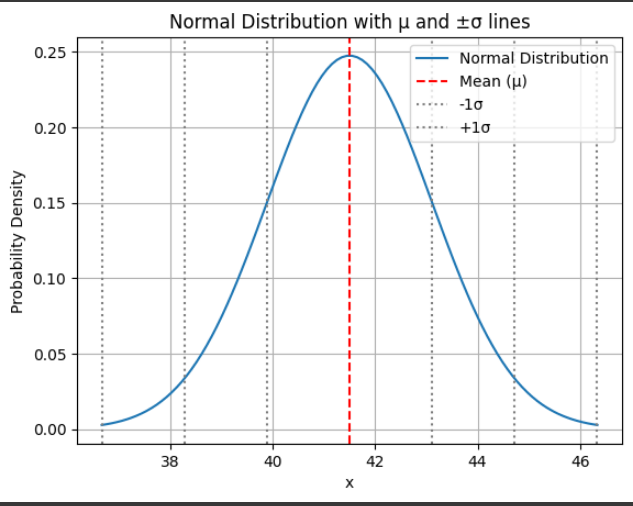
\includegraphics[width=0.75\linewidth]{normalDistro1d.png}
\end{center}

Previously we calculated the Maximum Likelihood Estimator for the variance (biased) and Maximum Likelihood Estimator for the mean. \\
The graph has 41.5 as the mean and $\hat{\sigma}^2_{MLE}=6.8$. The center in the distribution is representing the true mean (on average). But the spread of the plot (width, see dotted lines) is too narrowbecause it underestimates the true variance.

\end{solution}
\end{subtask}
\end{task}

\newpage

\begin{task}[points=9]{Non-Parametric Density Estimation}
Given the following dataset graph

\begin{center}
    \begin{tikzpicture}
      % Draw grid
      \draw[step=1cm,lightgray,very thin] (0,0) grid (7,7);
    
      \draw[->,thick] (0,0) -- (7.2,0) node[right] {width};
      \draw[->,thick] (0,0) -- (0,7.2) node[above] {height};
    
      \foreach \x in {1,2,3,4,5,6}
        \draw (\x,0.1) -- (\x,-0.1) node[below] {\x};
      \foreach \y in {1,2,3,4,5,6}
        \draw (0.1,\y) -- (-0.1,\y) node[left] {\y};
    
      % points
      \filldraw[black] (1,5) circle (2pt) node[above right] {A};
      \filldraw[black] (5,3) circle (2pt) node[above right] {B};
      \filldraw[red] (1,2) circle (5pt);
      \filldraw[cyan] (3,1) circle (5pt);
      \filldraw[green] (4,2) circle (5pt);
      \filldraw[pink] (6,1) circle (5pt);
      \filldraw[cyan] (6,4) circle (5pt);
      \filldraw[yellow] (5,5) circle (5pt);
      \filldraw[orange] (3,5) circle (5pt);
      \filldraw[red] (2,6) circle (5pt);
    \end{tikzpicture}
\end{center}

depicting the fruit colors red, orange, blue, green, pink and yellow with their corresponding width and height features. For example, the feature values of the pink fruit are (6, 1). In this task, we will apply the k-Nearest Neighbor (kNN) method to classify the color of fruit A and B shown in the graph, using a kernel to measure the similarity between data points. The Euclidean distance is defined as $d(\boldsymbol{x}, \boldsymbol{y}) = \left\| \boldsymbol{x} - \boldsymbol{y}\right\|_2$ and is used to define the distance in the feature space. For the entirety of this task, the hyperparameter will be $k = 3$ for the kNN method. 


\begin{subtask}[points=7]

Assume that the kernel is Gaussian $k(\boldsymbol{x}, \boldsymbol{y}) = e^{-\alpha d(\boldsymbol{x}, \boldsymbol{y})^2}$, classify the color of fruit A with $\alpha=0.2$. 

List the nearest neighbors of A and B that are relevant for the classification, including their Euclidean distances and corresponding similarity scores (kernel values). Then, use the kernel values to determine the predicted class for each point.

\begin{solution}

With $k=3$, we will need the $3$ nearest neighbors for points $A$ and for $B$. The three closest neighbors for $A$ are the two red fruits and one orange fruit:
\textbf{Point A: $(1, 5)$}
\begin{itemize}
    \item $x_{\text{red}1}=(2, 6)$ : Distance: $\sqrt{2}$; Kernel Value: $0,6703$ 
    \item $x_{\text{orange}}=(3, 5)$ : Distance:$2$; Kernel Value: $0,4493$
    \item $x_{\text{red}2}=(1, 2)$ : Distance: $3$; Kernel Value: $0,1653$
\end{itemize}

Kernel Sums for Point A:
\begin{itemize}
    \item Class red: $0,6703+0,1653=0,8356$
    \item Class orange: $0,4493$
    \item Point A is assigned to class red.
\end{itemize}

\textbf{Point B: $(5, 3)$}
\begin{itemize}
    \item $x_{\text{green}1}=(4, 2)$ : Distance: $\sqrt{2}$; Kernel Value: $0,6703$ 
    \item $x_{\text{blue}1}=(6, 4)$ : Distance: $\sqrt{2}$; Kernel Value: $0,6703$
    \item $x_{\text{yellow}}=(5, 5)$ : Distance: $2$; Kernel Value: $0,4493$
\end{itemize}

Kernel Sums for Point b:
\begin{itemize}
    \item Class green: $0,6703$
    \item Class blue: $0,6703$
    \item Class yellow: $0,4493$
    \item Point B is assigned either to green or blue. Because it wasn't defined how to handle tie-breaks, we will leave it at that.
\end{itemize}

\end{solution}
\end{subtask}

\begin{subtask}[points=2]
What problem arises if we use the kernel to weight the neighbors’ contributions and set $\alpha = 20$ or higher? How does this affect the classification?
\end{subtask}

\begin{solution}

If we look at some examples, and calculate the kernel with a distance of $\sqrt{2}$, and $2$, we will see the problem that arises.\\
With $\alpha=20$ the kernel value for $\sqrt{2}$ is $4,248354255*10^{-18}$ and the kernel value for distance $2$ is  $1,804851388*10^{-35}$. If we just look at the exponent, we see that the closest neighbor will contribute a lot, and somewhat close neighbors will be very small.  This kann lead to overfitting, because it is way too sensitive.

\end{solution}
\end{task}

\newpage

\begin{task}[points=16]{Bayesian Estimation}

Given is a dataset \( \mathcal{D} = \{x_1, x_2, \dots, x_n\} \). Each \( x_i \in \mathbb{R} \) is drawn independently from a Gaussian distribution with \textbf{unknown mean} \( \mu \) and \textbf{known variance} \( \sigma^2 \). That is,

\[
x_i \sim \mathcal{N}(\mu, \sigma^2), \quad \text{for } i = 1, \dots, n
\]

We want to estimate the distribution of the mean $ p(\mu \mid \mathcal{D}) $ using Bayesian Estimation. We define the prior over $\mu$ by another Gaussian distribution:
\[
\mu \sim \mathcal{N}(\mu_0, \tau^2)
\]
\begin{subtask}[points=2]{}
    Write the likelihood function $p(\mathcal{D} \mid \mu)$ and the prior $p(\mu)$.
\end{subtask}

\begin{solution}

The likelihood function would be:
\[p(D|\mu)=\Pi^n_{i=1} p(x_i|\mu)\]
beause the ddatapoints are drawn independently. \\
The prior is given in the task description:
\[p(\mu)=\frac{1}{\sqrt{2\pi\tau^2}}\exp (-\frac{(\mu-\mu_0)^2}{2\tau^2})\]

\end{solution}

\begin{subtask}[points=2]


\textbf{1)} Under the Gaussian prior, what type of distribution does the posterior $ p(\mu \mid \mathcal{D})$ assume? 

\textbf{2)} How is this concept called in the lecture?
\end{subtask}

\begin{solution}

\begin{enumerate}
    \item The assumption made is, that the posterior is also a Gaussian.
    \item Conjugate priors
\end{enumerate}

\end{solution}

\begin{subtask}[points=12]

\begin{programmingtaskbox}
Complete the corresponding section of the notebook as part of this task.
\end{programmingtaskbox}
    In this task, we are going to implement Bayesian estimation for a Gaussian with unknown mean and known variance in Python. The update rules for the mean and variance of our posterior look like this:

    \begin{align}
        \mu_{n} &= \frac{\sigma^{2} \cdot \mu_{0}}{\sigma^{2}+n\cdot\sigma_{0}^{2}} + \frac{\sigma_{0}^{2}\cdot \sum_{i=1}^{n} x_i}{\sigma^{2}+n\cdot\sigma_{0}^{2}}\\
    \end{align}
        \text{We substitute the sum $\sum_{i=1}^{n} x_i$ with $\sum_{i=1}^{n} x_i = n \cdot \frac{1}{n} \sum_{i=1}^{n} x_{i} = n \cdot \Bar{x} = n \cdot \mu_{MLE}$ }\\
    \begin{align}
        \mu_{n} &= \frac{\sigma^{2} \cdot \mu_{0}}{\sigma^{2}+n\cdot\sigma_{0}^{2}} + \frac{\sigma_{0}^{2}\cdot n \cdot \mu_{MLE}}{\sigma^{2}+n\cdot\sigma_{0}^{2}}\\
        \sigma_{n}^{2} &= \left(\frac{1}{\sigma_{0}^{2}} + \frac{n}{\sigma^{2}}\right)^{-1} 
    \end{align}

    You are not allowed to import any additional functionality. Begin by loading the file \texttt{GaussianBayesianEstimation.npy}. Here are some rough guidelines for the implementation of this task:
    \begin{itemize}
        \item Load the file \texttt{GaussianBayesianEstimation.npy} which contains a numpy array 
        \item Initialize the parameters for the Gaussian Likelihood with unknown mean $\mu$ and known variance $\sigma^{2}=4$  
        \item Initialize the parameters for the Gaussian Prior with $\mu_{0}=0$ and variance $\sigma_{0}^2=9$. Since we have no concrete prior information about the dataset we initialize a weakly informative prior with high variance.
        \item Implement the update rules for the parameters of the posterior.
        \item Compute the parameter values for the posterior as well as the maximum likelihood estimator for the mean for $n \in \{1, 2, 5, 10, 100, 1000\}$, where n is the number of data points, and plot the prior, posterior as well as the maximum likelihood estimate of the mean for each value of n resulting in 6 plots.
    \end{itemize}



\begin{figure}[h]
    \centering
    \includegraphics[width=0.5\linewidth]{Task4c)_Plot_Example.png}
    \caption{Resulting Plot for n=1}
    \label{fig:task4c-plot-n1}
\end{figure}

    Now using the plots, describe the observed behavior. What are the main differences between maximum likelihood estimation and Bayesian estimation?
\end{subtask}

\begin{solution}

In the Prior and Posterior for $N=1$, the posterior is pulled towards the prior, which is why it is not matching with the MLE line. Similar behaviour is in $N=2$\\
In $N=5$ and $N=10$ the posterior mean is closer to the MLE. It pulls away from the prior, because more datapoints are used.\\
The posterior in $N=100$ and $N=1000$ is aligning with the MLE, and the influence of the prior is very little.\\

\begin{center}
    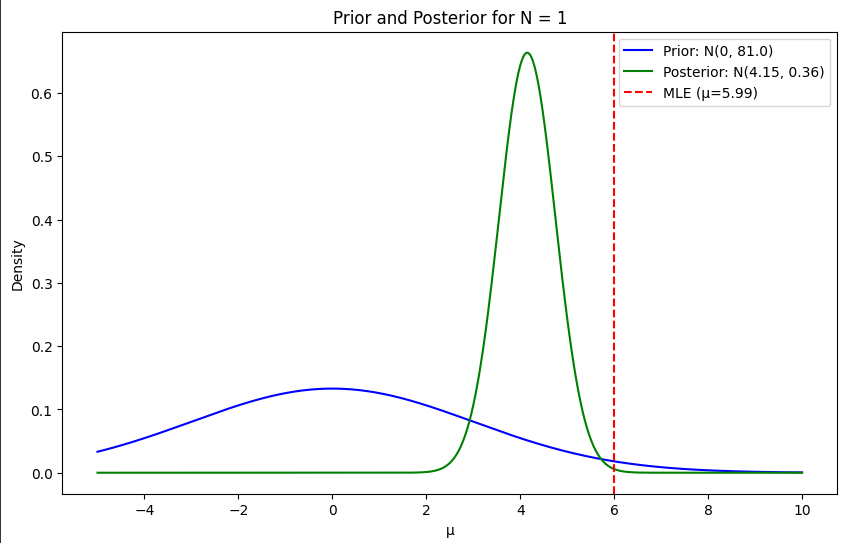
\includegraphics[width=0.75\linewidth]{priorAndPosteriorN1.png}
\end{center}

\underline{\textbf{Pictures of the other plots (N=2, 5, 10, 100, 1000) will be provided in a zip}}

\textbf{Differences between MLE and Bayesian estimation}

The result of the MLE is a point (in $N=1000$ its 5.04 for example). The result of the Bayesian estimation is a distribution. This means, that the posterior variance represents the confidence in the estimation, but MLE does not, due to its point characteristic. \\

Depending on the amount of data provided, the two estimators behave differently. For smaller data amounts, MLE is fitting to much to noise and becomes unstable. The bayesian estimation is influenced by the prior, which makes it more stable. With more data amounts MLE is accurate, and bayesian estimation approaches the MLE.



\end{solution}
\end{task}

\newpage

\begin{task}[points=6 + 4]{Expectation Maximization for Gaussian Mixture Models}
\begin{programmingtaskbox}
Complete the corresponding section of the notebook as part of this task.
\end{programmingtaskbox}

\textbf{For the entirety of this task, no additional packages are allowed other than the ones already given.}


In this task, we would like to implement the Expectation Maximization (EM) algorithm to fit a Gaussian Mixture Model (GMM) to a dataset. You have learnt from the lecture about GMM - modeling data using a sum of individual Gaussian distributions. However, the challenge is estimating the parameters of these Gaussians, as the MLE solution for this is more complex than the case of a single Gaussian. (Lecture 3, Slide 51). 

\textbf{Background about EM.}
The EM algorithm is a method for solving this problem. EM is an iterative method for finding maximum likelihood solutions for models with latent variables such as GMMs. In GMMs, the latent variables are the hidden mixture/cluster assignments. The algorithm has two main steps, which are repeated until convergence:
\begin{enumerate}
    \item Expectation step (E-step): In this step, we compute the probabilistic assignment of data points to the probability distributions. In other words, we want to compute the \textbf{responsibilities}, i.e., the probability that each data point belongs to each Gaussian component using the \textit{current parameters}.
    \begin{equation*}
    a_{nj} = p(j|x_n) = \frac{ \pi_j \mathcal{N}(x_n  | \mu_j, \sigma_j) }
                                { \sum_{i=1}^J \pi_i \mathcal{N}(x_n | \mu_i, \sigma_i) }.
    \end{equation*}
    \item Maximization step (M-step): Using the responsibilities computed from the previous E-step, we re-estimate the parameters (means, covariances, and mixing coefficients) of each Gaussian components. 
    \begin{equation*}
    \mu_j = \frac{ \sum_{n=1}^N a_{nj}x_n } { \sum_{n=1}^N a_{nj} }, \quad
    \sigma_j^2 = \frac{ \sum_{n=1}^N a_{nj}(x_n-\mu_j)(x_n-\mu_j)^T } { \sum_{n=1}^N a_{nj} },
    \quad \pi_j = \frac{ \sum_{n=1}^N a_{nj} } {N }.
    \end{equation*}
\end{enumerate}
An iteration of the EM algorithm consists of an E-step and a M-step. After each iteration, we evaluate the log likelihood with the new parameter estimates obtained from the last M-step and check for convergence. Below are some additional notes about the algorithm.
\begin{itemize}
    \item $x_n$ is a data point out of the dataset of N data points.
    \item In the expectation step, we want to compute the probability that each data point belongs to each Gaussian component. This means there will be $N*J$ $a_{nj}$ values to compute, assuming the dataset contain $N$ points and there are $J$ Gaussian components. Furthermore, because we are working with posterior probabilities, keep in mind that $ \sum_{j=1}^J a_{nj} = 1$ for each data point $x_n$.
    \item If you are unsure what mixing coefficient means, see Lecture 3, Slide 49.
    \item In the maximization step, the covariances are updated based on the \textbf{new means}. In other words, the new means have to be computed before the new covariances.
    \item You can check out Bishop, Chapter 9.2.2 if you still feel unsure about any details of the EM algorithm.
    \item You may have noticed that in order to start the first iteration of the algorithm, we need an initial estimate of the parameters for the Gaussian components. For this, we have provided the function \texttt{init\_EM()}, which will be used in task 4b).
\end{itemize}


\begin{subtask}[points=6,title=EM Implementation]

Implement the Expectation Maximization algorithm for Gaussian Mixture Models from scratch. More specifically, complete the following functions in the notebook:
    \begin{itemize}
        \item \texttt{expectation()} for the expectation step,
        \item \texttt{regularize()} for regularizing the covariance matrices in the maximization step,
        \item \texttt{maximization()} for the maximization step,
        \item \texttt{compute\_log\_likelihood()} for estimating the log likelihood.
        \item \texttt{em\_gmm()}, which leverages the previously implemented functions. 
    \end{itemize}
For your implementation, note the following:
\begin{itemize}
    \item To compute the multivariate normal probability density function you can use the function \texttt{multivariate\_normal} from \texttt{scipy.stats}. 
    \item {For the regularization, implement the function so that a small value is added to the diagonal entries of the covariance matrix, i.e. $\boldsymbol{\Sigma}_{\text{reg}}=\boldsymbol{\Sigma}+\sigma_{\text{min}}\boldsymbol{I}$. Make sure to use this in your EM implementation.}
    \item For the stopping criterion of \texttt{em\_gmm()}, check if the log likelihood has converged, i.e., the absolute difference in subsequent values is strictly below a certain threshold $\epsilon$.
    \item Aside from returning the mixture components and the responsibilities/posteriors, \texttt{em\_gmm()} should also return all the computed log likelihood values.
\end{itemize}

\begin{solution}

\end{solution}

\end{subtask}

\begin{subtask}[points=4]
We now want to test the implemented algorithm on the provided dataset \texttt{clustering\_dataset.npy}. Set the number of mixture components to 3 and $\epsilon$ to 0.001. Initialize the mixture components using the provided helper function \texttt{init\_EM()}. Plot the log likelihood values at every iteration. After that, complete \texttt{plot\_results()} to visualize the final clustering result along with the mixture components in a single plot. 

Your visualization should show each data point's corresponding mixture component. To simplify the visualization, from the soft assignment result of EM-GMM, assign each data point to the component with the highest corresponding responsibility/posterior (hard assignment).

\textbf{Hint:} For the mixture components, think about how you can visualize them when you are working with 2D data points. Lecture 1b, Slide 23 can be helpful.
\end{subtask}

\begin{solution}

\end{solution}
\end{task}

\newpage

\begin{task}[points=6]{Fisher's Linear Discriminant}
\begin{subtask}[points=3]{}
From the lecture slides, following optimzation problem is known
\[
\mathbf{w}^* = \arg\max_{\mathbf{w}} \left( \mathbf{w}^T \mathbf{m}_1 - \mathbf{w}^T \mathbf{m}_2 \right)^2
\]
Show mathematically why the optimal solution for \( \mathbf{w}^* \) grows without bound (i.e., the norm \( \|\mathbf{w}\| \to \infty \)) if no constraint is placed on \( \mathbf{w} \). What does this imply about the nature of this optimization problem?
\end{subtask}
\begin{solution}


First we will re-formulate the problem.

\begin{align*}
    (w^Tm_1-w^T-m_2)^2 = (w^T(m_1-m_2))^2
\end{align*}
 We define $m_\delta=m_1-m_2$.
 \[w^*=\arg \max_w (w^Tm_\delta)^2\]

we want to maximize the dot product, to do that, we want $w$ to be in the same direction of $m_\delta$, because this is the perfect condition to scale. Because $w$ is unbounded, we can just make it as long as we want. It grows without bound, because there is always a larger possible length that can be taken.\\

\textbf{What does this imply about the nature of this optimization problem?}\\

Without limiting the length of the vector, there is no actual best solution.

\end{solution}

\begin{subtask}[points=3]{}
In this task, at least one answer is true for each multiple-choice question. Each wrong answer results in a minus point. The minimum amount of points is 0. You may explain your choice, if you are unsure with your answer, but note that choosing the wrong answer with a sound explanation will only result in no minus point.

\begin{enumerate}
\item Which of the following is true for Fisher's Linear Discriminant in the two-class case?

\begin{itemize}[label=\Square]
    \item Fisher's Linear Discriminant maximizes the distance between the means of the classes while minimizing the variance within each class.
    \item Fisher's Linear Discriminant assumes equal class-conditional distributions with diagonal covariance.
    \item Fisher's Linear Discriminant requires i.i.d. data in order to compute a meaningful linear classifier.
    \item A solution $\mathbf{w}^*$ exists for non-linearly separable data under Fisher's criterion.
\end{itemize}

\item Suppose the within-class covariance matrix $S_W$ is singular (not invertible). What is the implication for Fisher’s Linear Discriminant?
\begin{itemize}[label=\Square]
    \item The data is i.i.d.
    \item The solution $w$ cannot be computed.
    \item $S_B$ should be used instead.
    \item The entries of $S_W$ must be tweaked such that $S_W$ becomes invertible.
\end{itemize}
\end{enumerate}

\end{subtask}


\begin{solution}

\begin{enumerate}
    \item True Statements: Fisher's Linear Descriminant in the two-class case
    \begin{itemize}
        \item \textbf{Fisher's Linear Discriminant maximizes the distance between the means of the classes while minimizing the variance within each class}
        \item \textbf{A solution $w^*$ exists for non-linearly separable data under FIsher's criterion}\\ Explanation: Technically, a solution will be found in non-linearly separable data. It won't be a perfect solution, but it will be a solution.
    \end{itemize}
    \item True Statements: Implications for Fisher's Linear Discriminant within-class covariance matrix $S_W$ is singular.
    \begin{enumerate}
        \item \textbf{The solution $w$ cannot be computed} \\ 
        Explanation: The Fisher's Linear Discriminant is calculated with $w \propto S^{-1}_W (m_1-m_2)$. If the matrix is not invertible, it can not be computed. (Lecture 4 Slide 39)
    \end{enumerate}
\end{enumerate}

\end{solution}
\end{task}

\newpage 

\begin{task}[points=5]{LDA Implementation}
\begin{programmingtaskbox}
Complete the corresponding section of the notebook as part of this task.
\end{programmingtaskbox}
In this exercise, you will use the dataset ldaData.txt, containing 100 points. Each row corresponds to a point, where the first and second values are the features of a point respectively. The first 50 points belong to class C1, the remaining 50 belong to class C2.
\begin{subtask}[points=5]{}
Implement the Fisher linear discriminant in Python, i.e., plot the projection line of the data. You are allowed to use built-in functions for computing the mean, the covariance, eigenvalues and eigenvectors.

\begin{solution}

\end{solution}
\end{subtask}
\end{task}

\clearpage

\end{document}